\section{Data Exploration}

The dataset consists of 50.000 reviews and their corresponding review (1-4 for negative, 7-10 for positivie). 
In Figure~\ref{fig:data-dist} the split for both the training and test set can be found.
It can be noted that the distributions are about the same, meaning the dataset does not have an inherent bias towards positive or negative reviews.
An other interesting fact is that both review of score 1 and 10 are highly represented in the dataset in comparision to the other review scores.

\begin{figure}[ht!]
    \centering
  \subfloat[Test Review Distribution\label{fig:test-dist}]{%
       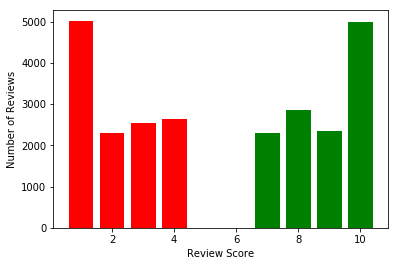
\includegraphics[width=0.5\linewidth]{figures/data-visualization/test_review_dist.png}}
    \hfill
  \subfloat[Train Review Distribution\label{fig:train-dist}]{%
        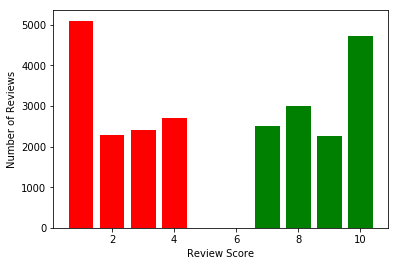
\includegraphics[width=0.5\linewidth]{figures/data-visualization/train_review_dist.png}}
  \caption{Test \ref{fig:test-dist} and train \ref{fig:train-dist} review frequency distribution.}
  \label{fig:data-dist} 
\end{figure}

When looking at the reviews and analyze the positive and negative reviews separately, we can see that the distribution of words differ, but many appear in both datasets, see Figure~\ref{fig:wordclouds}.

\begin{figure*}[ht!]
    \centering
  \subfloat[Negative wordcloud\label{fig:neg-wordcloud}]{%
       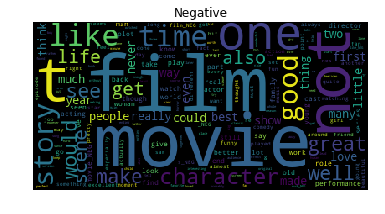
\includegraphics[width=0.5\linewidth]{figures/data-visualization/negative_wordcloud.png}}
    \hfill
  \subfloat[Positive wordcloud\label{fig:pos-wordcloud}]{%
        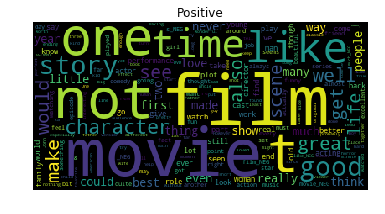
\includegraphics[width=0.5\linewidth]{figures/data-visualization/positive_wordcloud.png}}
  \caption{Wordclouds for the both negative \ref{fig:neg-wordcloud} and positive \ref{fig:pos-wordcloud} reviews.}
  \label{fig:wordclouds} 
\end{figure*}